\chapter{Refinement of the INTERLACE Business Logic Specification}
\label{ch:UpdateBLS}

\vspace{-1cm}
\begin{center}
Paolo Dini, Luca Carboni, Giuseppe Littera, and Chrystopher Nehaniv
\end{center}

\section{Context}
The business logic specification provided in Deliverable D2.1 \cite{INTERLACE_D21} concerns user-initiated transactions. Although this is a subset of all possible operations (initiated by the users or by the System) that a mutual credit system platform must support, it is a viable starting point for testing an initial executable CoreASIM model. D2.1 did not provide all the details of the transaction request operations, it left their specification at a fairly abstract level. This chapter provides the next step in the iterative refinement of the specification in the form of a detailed description of the Permissioning workflow, whose implementation as part of the CoreASIM model is then described in Chapter \ref{ch:CoreAsimImplementation}.

The description of the Permissioning iterative refinement relies mainly on graphical depictions of the variables and functions involved. As this reflects the process that was used to build a shared understanding within the INTERLACE team itself, it is hoped that it will also make it easier for newcomers to the INTERLACE open source community to understand the implementation.

\begin{figure}[htbp]
\centering
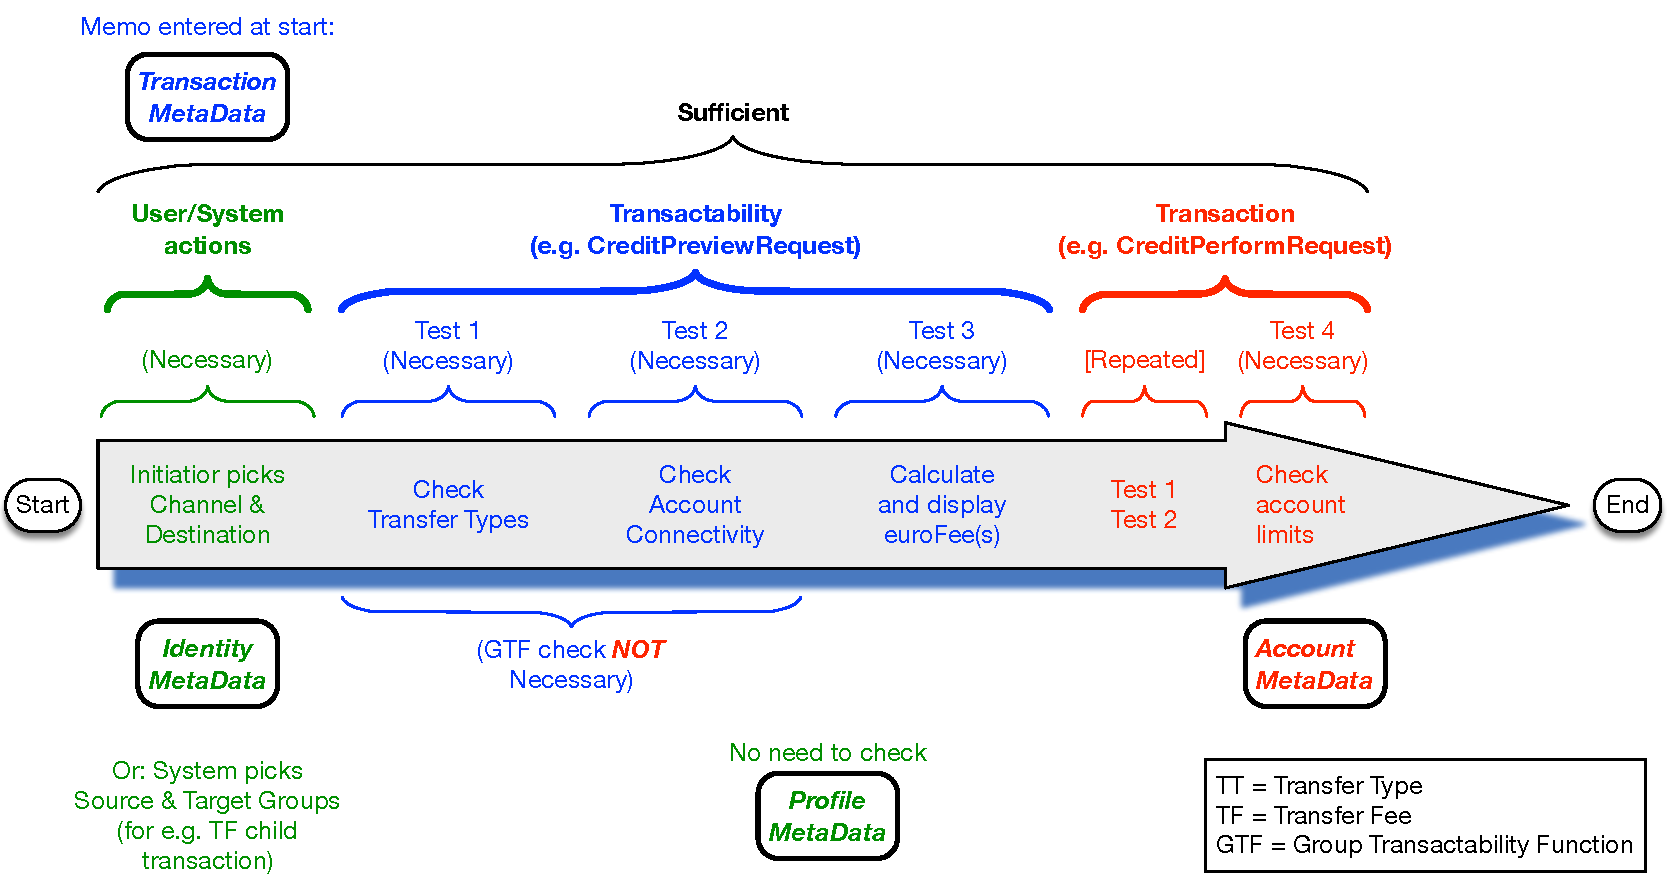
\includegraphics[width=16cm]{Figures/Transactability_Workflow}
\caption{\small\textbf{High-level workflow of the Permissioning process for user- or system-initiated transactions}}
\label{fig:transactabilitywkflow}
\end{figure}

\section{Overview}
Figure \ref{fig:transactabilitywkflow} shows the high-level view of the process, including how example PreviewRequest and PerformRequest rules specified in D2.1 map onto it. The process can be seen to start on the left of the figure, when a user or the System initiates the request for a transaction. The request must pass the three tests shown: Transfer Types, Account Connectivity, and MetaData. Upon successful completion of these three tests, the user is shown a preview screen that summarizes all the transaction data. When the user issues the command to proceed, the three tests are repeated and a final test on the account limits (e.g.\ sufficient funds) performed. If also this fourth test is passed, the transaction is executed. We now describe each step in detail.

\section{Permissioning Model Taxonomy}
\subsection{Groups}
The original Sardex system divides its users into 29 different types, called `groups'. This generates a great deal of complexity that is drastically reduced in the INTERLACE version of the platform. The new user type taxonomy involves only 9 groups, as shown in Table \ref{tab:groups}.

%\setcounter{table}{0}
\setlength{\tabcolsep}{10pt}
\begin{table}[htbp]
\begin{centering}
\small
{
\begin{tabular}{| l | l | }
\hline
\textbf{Group}	& \textbf{Description} \\
\hline
$welcome$ & User who has joined and signed the contract, but has not yet been cleared to start trading \\
\hline
$retail$ & Retailer who can \emph{only} participate in B2C operations (not B2E and not B2B) \\
\hline
$company$ & Company, which could be a retailer, that can use B2E and B2B but \emph{not} B2C \\
\hline
$full$ & Has all the functions of $retailer$ and of $company$ \\
\hline
$employee$ & Employee of $company$ or of $full$ \\
\hline
$on$\_$hold$ & User whose privileges have been suspended (for whateve reason) \\
\hline
$consumer$ & Person not registered to the circuit who can only interact through B2C Use Case 2 \\
\hline
$consumer$\_$verified$ & $consumer$ who has registered and can now also purchase with SRD (B2C Use Case 3)  \\
\hline
$MNGR$ & Manager of the circuit (e.g.\ Sardex S.p.A.) acting as $company$ rather than $SysAdmin$ \\
\hline
\end{tabular}
}
\caption{\small\textbf{New user types (groups) for the INTERLACE platform}}
\label{tab:groups}
\end{centering}
\end{table}

$SysAdmin$ is not defined explicitly as a group, in this model, although technically it too is a user type. $SysAdmin$ has special privileges, some of which are discussed where relevant in what follows.

\subsection{Accounts}
As shown in Table \ref{tab:accounts}, the accounts implemented in the model reflect the current operations of the Sardex system and the needs of a wide range of business operations and interactions. Some of the account types, for example MIRROR, may be phased out as the high-level architecture of the family of Sardex circuits grows and different algorithms replace the current strict controls on the balance of payments between different circuits.


%\setcounter{table}{0}
\setlength{\tabcolsep}{10pt}
\begin{table}[htbp]
\begin{centering}
\small
{
\begin{tabular}{| l | l | }
\hline
\textbf{Account}	& \textbf{Description} \\
\hline
$CC$ & Standard Sardex credits (SRD) account \\
\hline
$DOMU$ & SRD account used for larger operations, such as for real estate or capital equipment\\
\hline
$MIRROR$ & Account controlled by $MNGR$, used for inter-circuit purchases \\
\hline
$Income$ & Statistical EUR account owned by $retail$ or $full$ that collects B2C payments\\
\hline
$Prepaid$ & Stastical EUR account from which the 2\% child B2C transaction fee is drawn \\
\hline
$Bisoo$ & Statistical EUR account used by $consumer$ to pay into Income \\
\hline
$Topup$ & Statistical EUR account used by $MNGR$ to recharge $retail$'s Prepaid account upon receipt of \\
&\hspace{0.5cm} EUR payment. It is recharged back to zero gradually with each B2C transaction. \\
\hline
\end{tabular}
}
\caption{\small\textbf{New user types (groups) for the INTERLACE platform}}
\label{tab:accounts}
\end{centering}
\end{table}


\subsection{Currencies and Channels}
As shown in Figure \ref{fig:currchan}, the Sardex/INTERLACE platform supports transactions in both Sardex credits (SRD) and Euros (Euro) over two kinds of channels. `Service' refers to transactions mediated either by a computer (web application) or a mobile phone (either a web application or a phone App). `POS' means `Point of Sale' and refers to the standard terminal used by retailers that accepts credit or debit cards, through which SRD transactions can be routed via an API. The figure also shows the four possible $\{ currency, channel \}$ combinations that we need to support in the definition and implementation of the permissioning tests discussed in the next sections.

\begin{figure}[htbp]
\centering
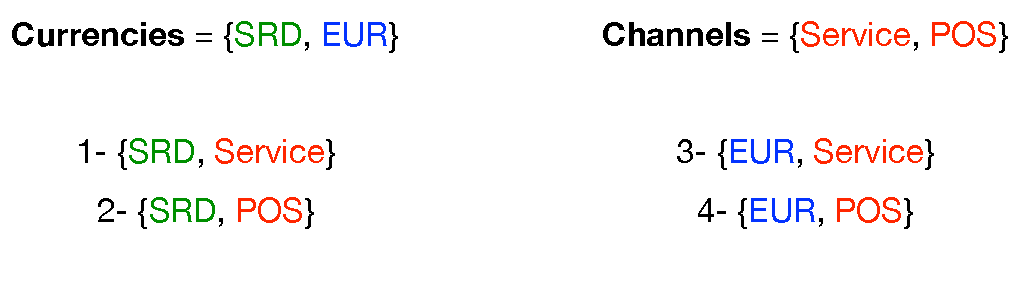
\includegraphics[width=10cm]{Figures/Curr_Chan}
\caption{\small\textbf{Currencies and channels supported by the platform}}
\label{fig:currchan}
\end{figure}

\subsection{Interaction Levels}
The interactions between circuit participants can be described from different points of view that correlate loosely to a stack view of the system. As shown in Figure \ref{fig:stack}, it is helpful to identify qualitatively the different levels of such a stack, acknowledging that it is \emph{more} than a networking communication stack in terms of scope but \emph{less} than one in terms of precision. `A' and `B' refer to the Initiator and the Target of the transaction, which do not necessarily correspond to the Buyer and the Seller.

\begin{figure}[htbp]
\centering
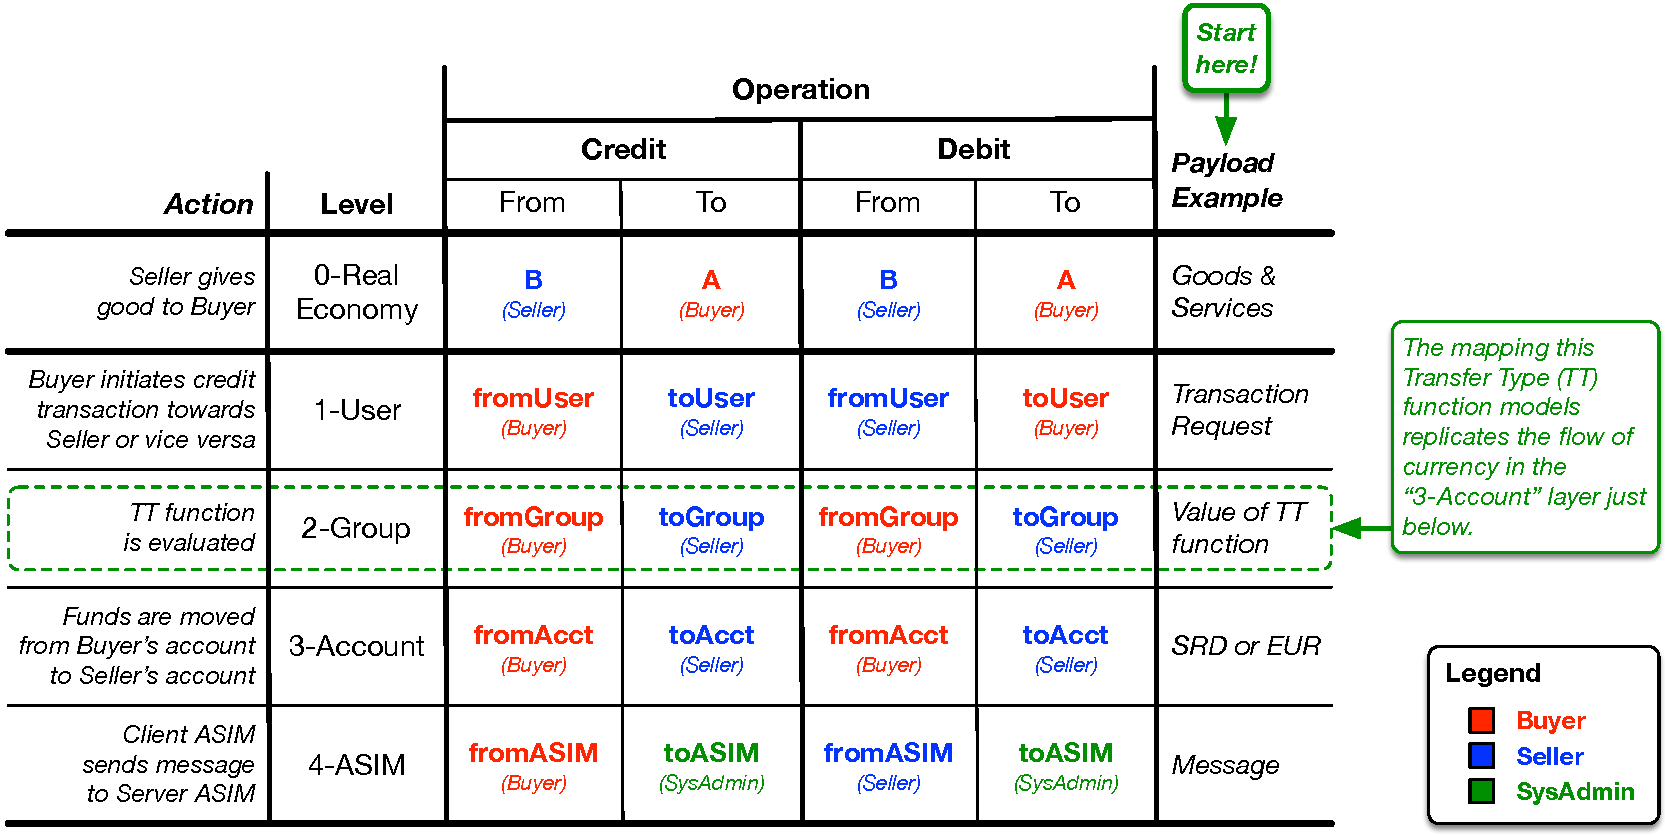
\includegraphics[width=9cm]{Figures/Stack}
\caption{\small\textbf{Stack view of the INTERLACE communication, economic, and financial  interactions}}
\label{fig:stack}
\end{figure}

\begin{figure}[htbp]
\centering
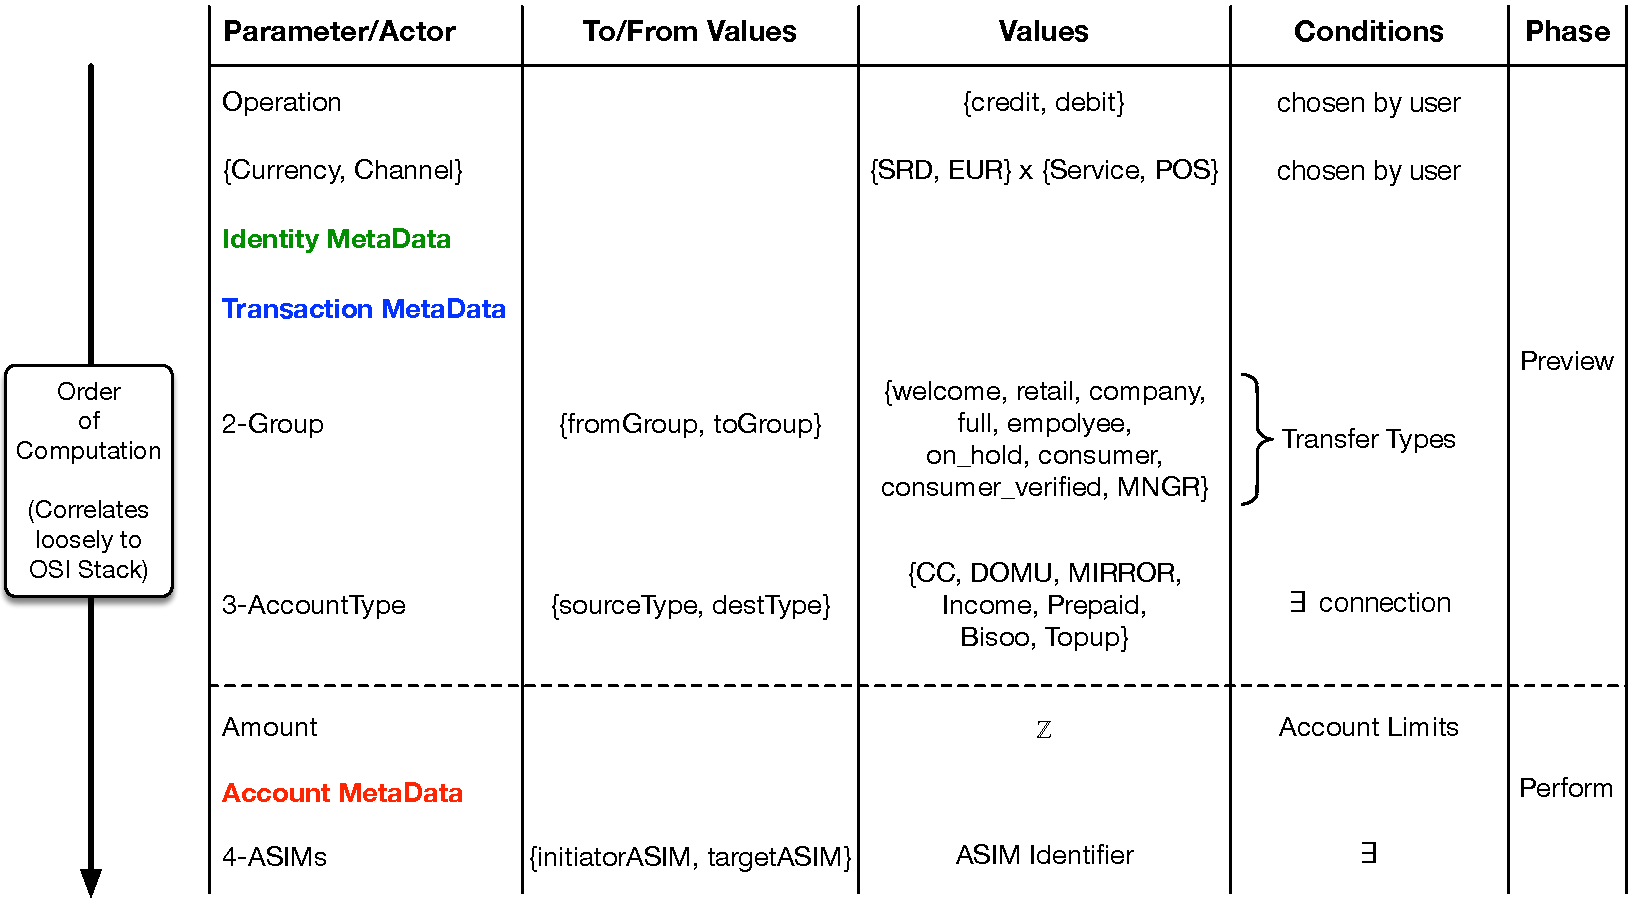
\includegraphics[width=17cm]{Figures/Vocabulary}
\caption{\small\textbf{Actors, parameters, levels, data structures, computational process, and conditions}}
\label{fig:vocabulary}
\end{figure}

Figure \ref{fig:stack} extends the two communication levels described in D2.1, but does so qualitatively. For the purposes of the implementation, we need a smaller set of levels but a more precise and specific vocabulary to identify the end-points of the transaction. Figure \ref{fig:vocabulary} shows this additional information as concerns levels 2, 3 and 4, which are labelled in the first column in the same way as in Figure \ref{fig:stack}, along with a great deal more information. In particular, this figure could be seen to integrate aspects of Figures \ref{fig:stack} and \ref{fig:transactabilitywkflow}, with the purpose of facilitating the conceptual understanding of the specification. `Groups' refer to user types, while `MetaData' to the parameters allocated to each user type or group. For example, the $\%$ of SRD accepted by a given user over 1000-EUR transaction values is a MetaData field of the Company group but not the Consumer\_Verified group.

\subsection{Visibility}
Figure \ref{fig:visibility} shows which groups ($toGroups$) are visible to which groups ($fromGroups$) by a `1' at the intersection of the $(row, column)$ corresponding to a choice of $(fromGroup, toGroup)$. For example, $company$ is visible to $employee$, meaning that $employee$ can do a search for $company$, but not vice versa. In this case $employee$ is not visible due to privacy legislation.

In general, transactability correlates to visibility. However, there is not a strict 1-1 relationship between them. For the example of a $company$ paying its own $employees$ as part of the B2E programme, $employee$ remains invisible to a search, but $company$ has the $username$ of the $employee$ and can perform a credit transaction to pay (part of) their salary.

\begin{figure}[H]
\centering
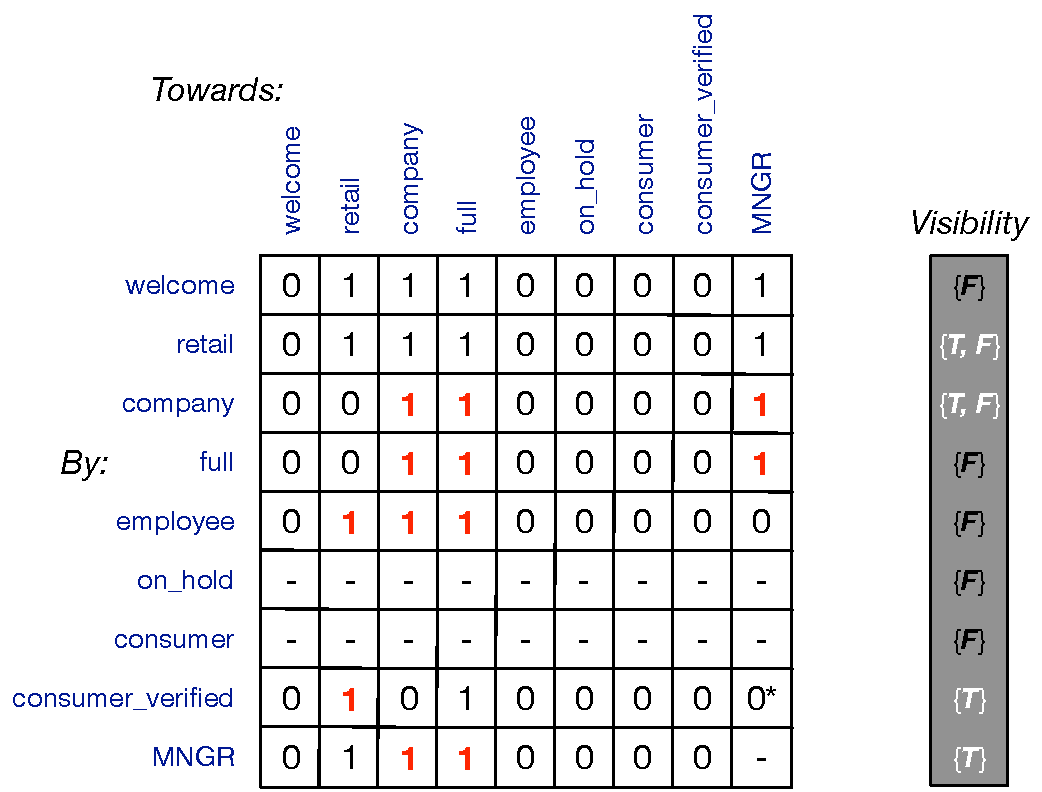
\includegraphics[width=12cm]{Figures/Visibility}
\caption{\small\textbf{Mutual visibility of different groups}}
\label{fig:visibility}
\end{figure}

On the right of Figure \ref{fig:visibility} we show that some groups are always invisible $\{ F \}$ others are always visibile $\{ T \}$, and others could be either $\{T, F\}$. For example, a company could be put in the shadow state if it has reached its maximum positive credit limit.

\subsection{B2C Operations}
This report extends the use cases covered by D2.1 by adding also the Business to Consumer (B2C) use cases. B2C was developed to increase the number and volume of transactions, i.e.\ the size of the Sardex economy, by extending the ability to transact in SRD to people not otherwise connected to the circuit. The principle involves offering the opportunity to $retail$ers to reward their EUR customers with an SRD rebate.

The amount of the reward is a percent, in SRD, of the amount in EUR paid by $consumer$ to $retail$, where the percent is set by $retail$ and it is an example of the $MetaData$ for this group. The reward is stored on a smart card that is offered to $consumer$ at the time of purchase. This is shown as a child transaction in B2C Use Case 2, Figure \ref{fig:B2C1}.

\begin{figure}[htbp]
\centering
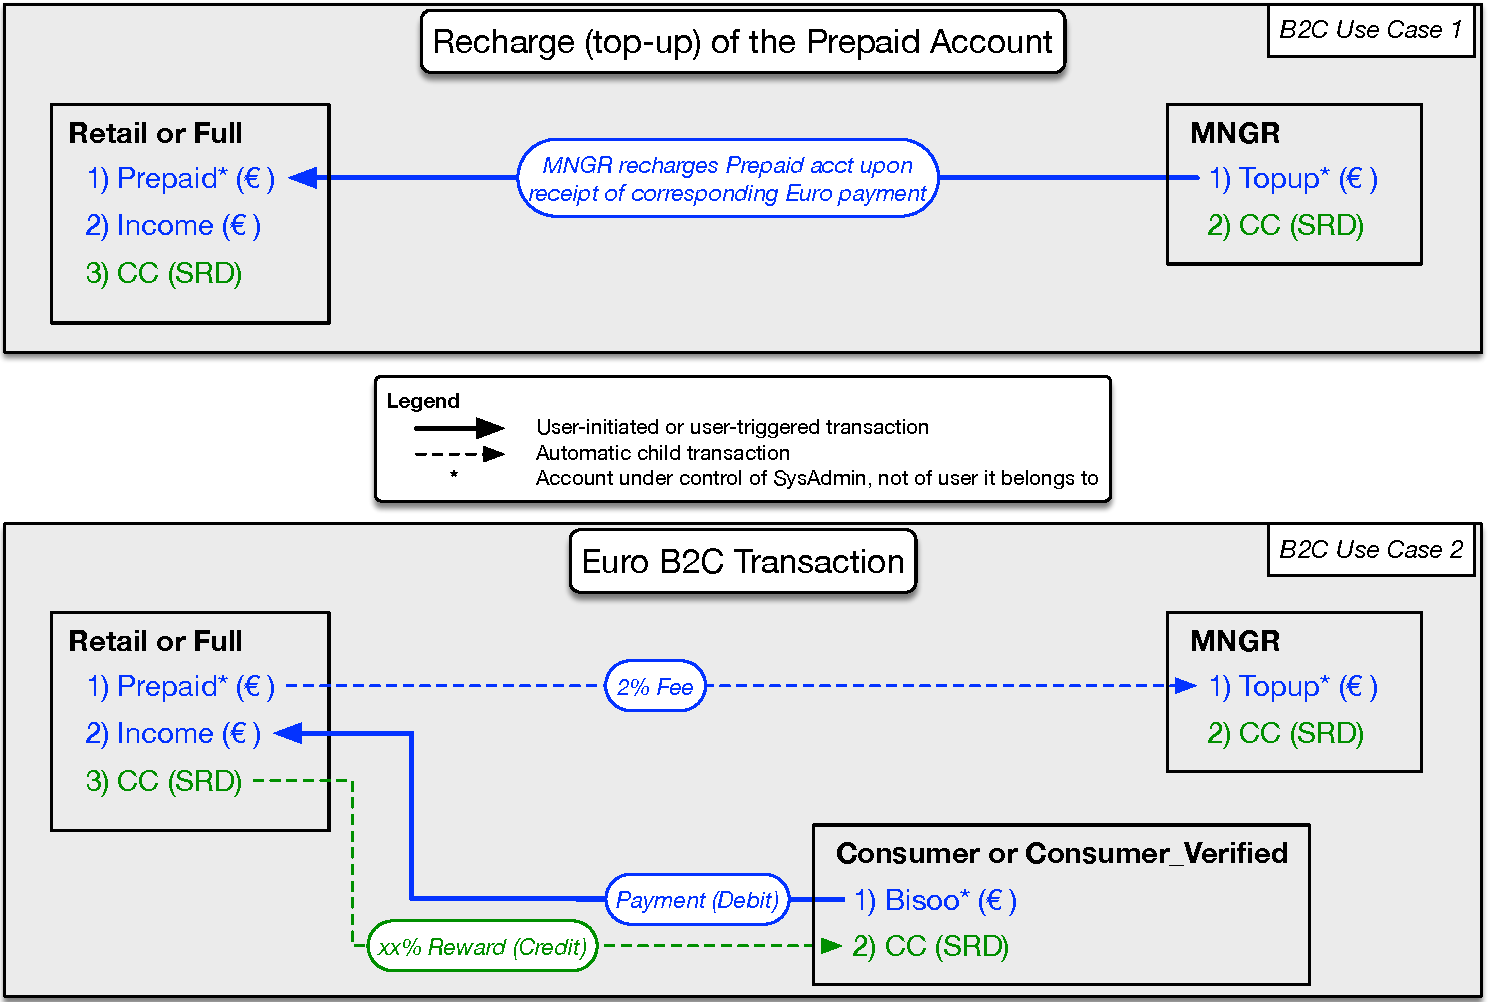
\includegraphics[width=15cm]{Figures/B2C1}
\caption{\small\textbf{Recharging of $retail$'s Prepaid account and standard B2C EUR transaction}}
\label{fig:B2C1}
\end{figure}

Use Case 2 also involves a second child transaction, a 2\% fee, in EUR, paid from $retail$'s Prepaid account to $MNGR$'s Topup account. The asterisks next to these account names, in the figure, indicate that these two accounts are \emph{owned} by these two users but are not \emph{controlled} by them. They are controlled by $SysAdmin$. These EUR accounts are `statistical' rather than `real', meaning that they simply keep track of actual EUR amounts but do not themselves hold Euros. Sardex S.p.A. would need to be a bank for that to be possible. For Use Case 2 to be executable, for a given $retail$er, its Prepaid account needs to have sufficient funds. When it runs out of statistical Euros, $retail$ can pay $MNGR$ some amount of Euros using any of the standard payment systems, through a bank or a payment service provider like PayPal. This triggers Use Case 1, also shown in Figure \ref{fig:B2C1}.

\begin{figure}[htbp]
\centering
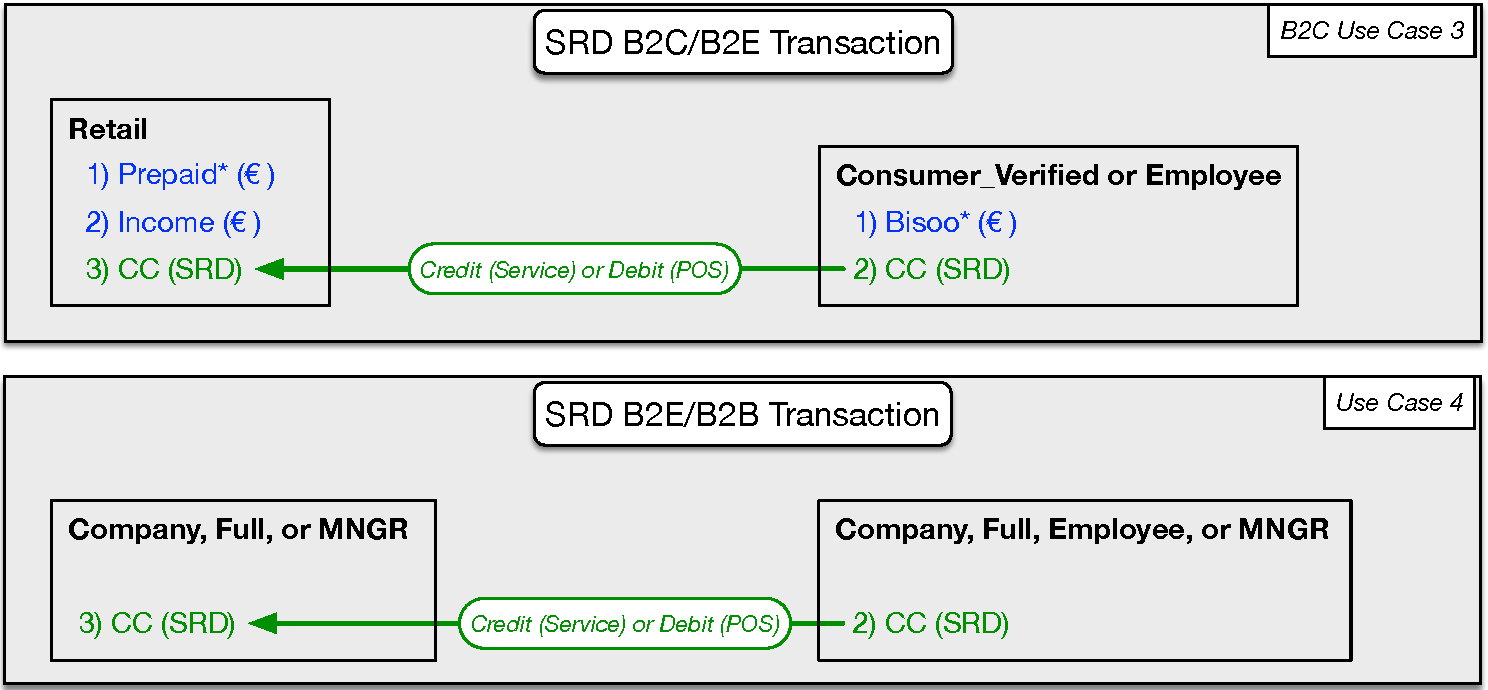
\includegraphics[width=15cm]{Figures/B2C2}
\caption{\small\textbf{B2C SRD transaction}}
\label{fig:B2C2}
\end{figure}

Figure \ref{fig:B2C2} shows the SRD transaction a $consumer$ can perform, i.e.\ the spending of the SRD accumulated as rewards, once they have registered and have become $consumer$\_$verified$.

\subsection{Initial Account State}
Figure \ref{fig:Initial_Acct_Sets} shows the initial allocation of accounts to the different user groups. The allocation is `initial' because  depending on the history of a given user the number of its accounts could change. For legal reasons, as a general principle \emph{change} can only mean \emph{increase}. In other words, once a user has become the owner of an account it can never be taken away from them, even if its access to it is, for example, suspended due to misbehaviour.

Another example is a $retail$ user who upgrades to $full$ and a year later changes its mind and goes back to $retail$. It will retain its DOMU account even if it won't be able to use it anymore.

\begin{figure}[htbp]
\centering
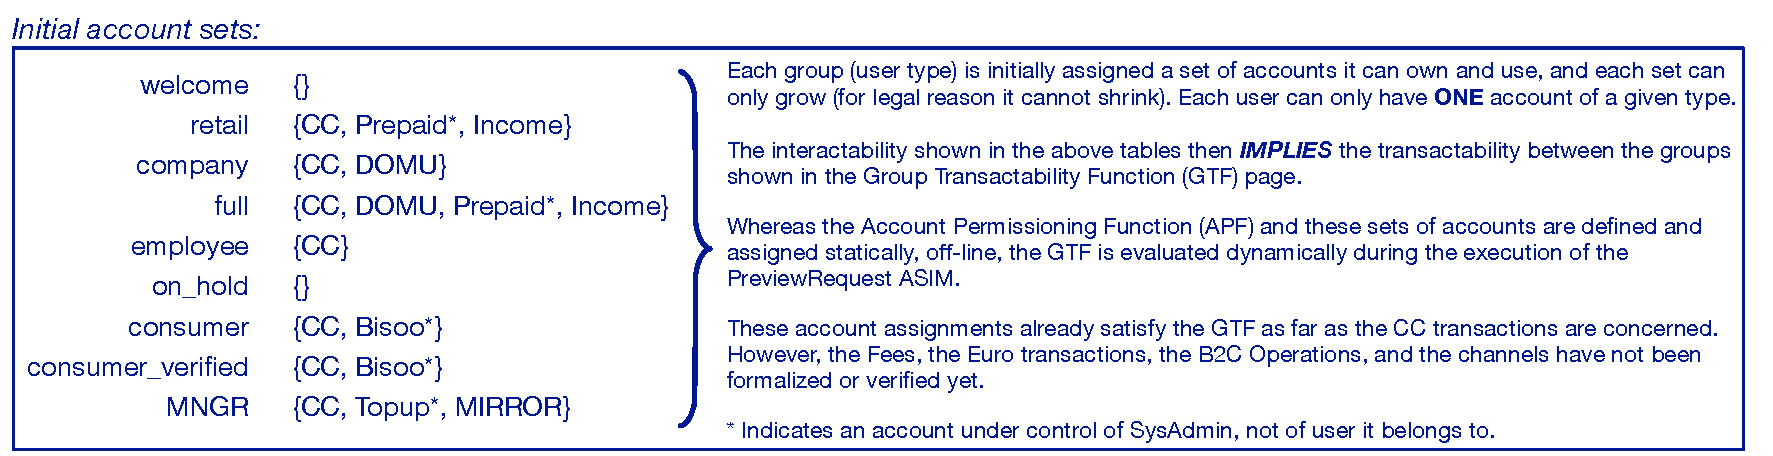
\includegraphics[width=17.5cm]{Figures/Initial_Acct_Sets}
\caption{\small\textbf{Initial account sets for different user groups \textcolor{red}{(THIS FIGURE WILL BE UPDATED)}}}
\label{fig:Initial_Acct_Sets}
\end{figure}

\section{Transactability Tests}
\subsection{Transfer Types}
As shown in Figure \ref{fig:transactabilitywkflow}, the first test for transactability involves so-called Transfer Types. Transfer Types are mathematical functions of the source groups ($fromGroups$) whose values are sets of target groups ($toGroups$). There is one different function for each combination of ordered pairs $(x, y)$, where $x \in \{ credit, debit \}$ and $y \in \{ SRD, EUR \}$, leading to four different functions. More formally,

\begin{align}
TT^{Credit,SRD}\colon &Groups\ \rightarrow\ Groups \times Groups \times \cdots \times Groups \\
TT^{Debit,SRD}\colon &Groups\ \rightarrow\ Groups \times Groups \times \cdots \times Groups \\
TT^{Credit,EUR}\colon &Groups\ \rightarrow\ Groups \times Groups \times \cdots \times Groups \\
TT^{Debit,EUR}\colon &Groups\ \rightarrow\ Groups \times Groups \times \cdots \times Groups,
\end{align}
where
\begin{align}
Groups &= \{ welcome, retail, company, full, employee, on\text{\_}hold,  \nonumber \\
		& \qquad\qquad\qquad\qquad\qquad\qquad\qquad
			consumer, consumer\text{\_}verified, MNGR \}.
\end{align}
If, with an abuse of notation and shamelessly overloading the terminology, we define for convenience the following target groups as different ``transfer types''
\begin{align*}
TT_1 &= \{ retail \},		&& TT_2 = \{ retail, company \},		&& TT_3 = \{ company, employee \} \\
TT_4 &= \{ company \},	&& TT_5 = \{ MNGR \},			&& TT_6 = \{ full \},
\end{align*}
we can now express the four functions as the following tables:

\setlength{\tabcolsep}{10pt}
\setlength\extrarowheight{3pt}
\begin{table}[htbp]
\begin{centering}
\small
{
\begin{tabular}{ r | c | c | c | c |}
\textbf{Group}	& $\bm{TT}^{\bm{Credit,SRD}}$ & $\bm{TT}^{\bm{Debit,SRD}}$ 
			& $\bm{TT}^{\bm{Credit,EUR}}$ & $\bm{TT}^{\bm{Debit,EUR}}$\\
\hline
$welcome$	& $\emptyset$ 				& $\emptyset$	& $\emptyset$	& $\emptyset$	 \\[3pt]
\hline
$retail$		& $\emptyset$				& $TT_1$ 		& $\emptyset$	& $TT_1$	 \\[3pt]
\hline
$company$	& $TT_3 \cup TT_5 \cup TT_6$ & $TT_4$		& $\emptyset$	& $\emptyset$	 \\[3pt]
\hline
$full$		& $TT_3 \cup TT_5 \cup TT_6$ & $TT_6$		& $\emptyset$	& $TT_6$	 \\[3pt]
\hline
$employee$	& $TT_2 \cup TT_6$ 		& $\emptyset$	&$\emptyset$ 	& $\emptyset$	 \\[3pt]
\hline
$on$\_$hold$	& $\emptyset$				& $\emptyset$	& $\emptyset$	& $\emptyset$	 \\[3pt]
\hline
$consumer$	& $\emptyset$				& $\emptyset$	& $\emptyset$	&$\emptyset$ 	 \\[3pt]
\hline
$consumer$\_$verified$ & $TT_1 \cup TT_6$ 	& $\emptyset$	& $\emptyset$ 	& $\emptyset$	 \\[3pt]
\hline
$MNGR$ 		& $TT_2 \cup TT_3 \cup TT_5 \cup TT_6$ & $TT_2 \cup TT_5 \cup TT_6$ & $\emptyset$ & $\emptyset$	 \\[3pt]
\hline
\end{tabular}
}
\caption{\small\textbf{The four Transfer Types functions}}
\label{tab:TTs}
\end{centering}
\end{table}

\subsection{Account Connectivity}



\subsection{MetaData}


\subsection{Group Transactability Functions}


\section{Account Limit Tests}











